%!TEX root = ./main.tex
\chapter{Approach
\label{chapter:approach}}

To achieve the goal of enhancing the traffic preselection of \gls{FACT} with knowledge about the past stability and popularity characteristics, the following three steps are planned for extending \gls{FACT} as illustrated in figure  \ref{fig:FACT}.

In a first step, a network service detector (server socket detector) is  implemented. 
The challenge of the network service detection lies in the fact  that the flow-level data does not provide enough precise timing information to  determine which flow is originated from the client making it impossible to deduce the server's socket\citep{Schatzmann:Tracing}. 
Therefore, the network service detection is achieved by the assumption that network services offered by servers act as concentrators in the sense that several clients have connections to this specific service. 
This approach bases on the work shown in \cite{Schatzmann:Dissection, Schatzmann:Mining, Schatzmann:Tracing} and is discussed in more detail in section \ref{section:socket_detection}.

\begin{figure}
	[t] \centering
	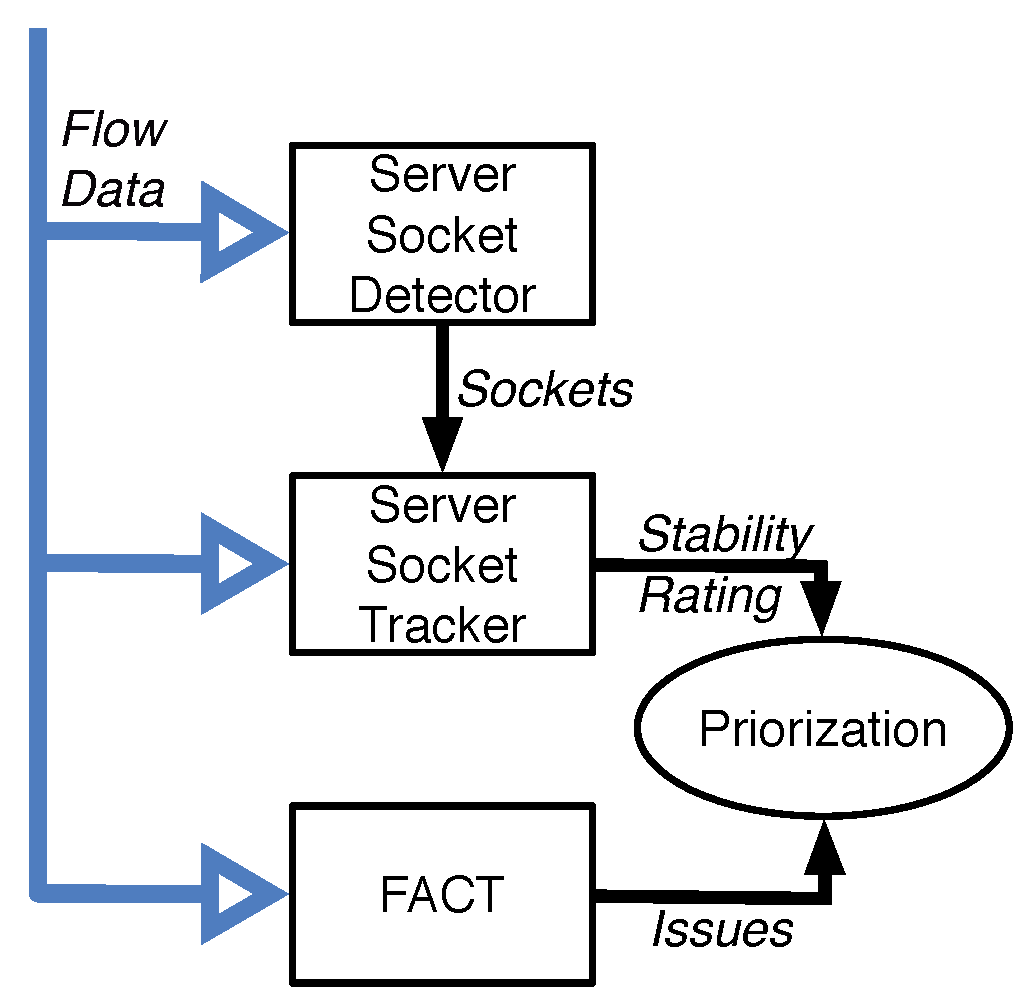
\includegraphics[width=8.5cm]{images/Approach_blockdiagram.eps}
	\caption{Interactions of new components with \gls{FACT}} 
	\label{fig:FACT} 
\end{figure}

In a second step, the previously detected network services are continually monitored and especially the successful and unsuccessful connection attempts are recorded by a network service monitoring engine (server socket tracker). This is detailedly covered in section \ref{section:socket_tracking}.
Furthermore, these information are then used to statistically characterize the network services by their visibility, popularity and stability as further outlined in section \ref{section:characterization}.

In a third step, FACT has to be extended to use these server sockets to smartly preselect the traffic which should be monitored. 
This adaption is explained in section \ref{section:ses_traffic_selection}. 
By choosing a set of suitable network services, \gls{FACT}'s sensibility to events and the observation coverage can be increased. 
However due to performance reason, the number of network services which are observed by \gls{FACT} have to be reduced. 
To this end, the properties of these observation sets has to be assessed, because they influence the observation capabilities of \gls{FACT}. 
Particularly, the sets' Internet address space coverage is a crucial property. 
With respect to FACT's goal of detecting remote network outages, it makes for example no sense to select only the most popular sockets if they are all located in the same network. 
Section \ref{section:ses_selection} is briefly addressing this problem.

%%%%%%%%%%%%%%%%%%%%%%%%%%%%%%%%%%%%%%%%%%%%%%%%%%%%%%%%%%%%%%%%%%%%%%%%%%%%%%%%
% SERVER SOCKETS
%%%%%%%%%%%%%%%%%%%%%%%%%%%%%%%%%%%%%%%%%%%%%%%%%%%%%%%%%%%%%%%%%%%%%%%%%%%%%%%%
\section{Server Sockets}
Since the Internet has moved from a research project to a widely used, public communication infrastructure, one of the critical success factors was its diversity with respect to network applications or services. This was heavily favored by the Internets layered design as described by the \gls{osi}.

Todays network applications ranges from traditional services as web, \gls{FTP} or mail to new and emerging services as video streaming and social networks. However, the terms \emph{network application} or \emph{network service} are overloaded and are used differently depending on the actual technical context.

By relying on flow-level data, information of layer 5-8 of the \gls{osi} are not available in the data set. Therefore, network services can be differentiated only by information of layer 3 and 4 of the \gls{osi}. For this reason, the following abstractions of a connection end-point are defined:

%%%%%%%%%%% SOCKET DEFINITION 			%%%%%%%%%%%%%%%%%%%%%%
\parbox{
\textwidth}{
\begin{defn}
	{\textbf{Socket}\\} A socket is uniquely defined by the triple (\textbf{IP address}, \textbf{IP protocol number} and \textbf{protocol port number}). In this context, a socket is only defined for IP protocol \gls{TCP}(6) and \gls{UDP}(17).
\end{defn}
}
%%%%%%%%%%% SERVER SOCKET DEFINITION 	%%%%%%%%%%%%%%%%%%%%%%
\parbox{
\textwidth}{
\begin{defn}
	{\textbf{Server Socket
	\label{def:serversocket}}\\} A server socket is a socket with at least one process listening to incoming connections and thus offering a network service. The lifetime of a server socket is not restricted to individual connections, but by the lifetime of the network service.
\end{defn}
}

%%%%%%%%%%% CLIENT SOCKET DEFINITION 	%%%%%%%%%%%%%%%%%%%%%%
\parbox{
\textwidth}{
\begin{defn}
	{\textbf{Client Socket}\\} A client socket is a socket which is only used to initiate and collate a connection to a server socket. Therefore, a client	socket is of temporary lifetime which is determined by the duration of the 	connection to the server socket.
\end{defn}
}

In spite of the use of the term \emph{server}, definition \ref{def:serversocket} is not only valid for classical server-client applications as \gls{HTTP}, \gls{FTP}, or \gls{SSH}, but also holds for \gls{p2p} applications. Furthermore, the definition allows completely symmetric server-server connections as for example \gls{NTP} as well.


%%%%%%%%%%%%%%%%%%%%%%%%%%%%%%%%%%%%%%%%%%%%%%%%%%%%%%%%%%%%%%%%%%%%%%%%%%%%%%%%
% DETECTION OF SERVER SOCKETS
%%%%%%%%%%%%%%%%%%%%%%%%%%%%%%%%%%%%%%%%%%%%%%%%%%%%%%%%%%%%%%%%%%%%%%%%%%%%%%%%
\section{Detection of Server Sockets
\label{section:socket_detection}}

% problem of detection with flow-level information (timing issue + flags)
Basically, a \gls{server socket} can be identified by the fact that a client opens a socket which initiates a connection to a \gls{server socket}. Usually, a \emph{client socket} port is chosen at random by his operating system and the \gls{server socket} port is statically allocated over the lifetime of network service process. Moreover, on each host a socket can only be assigned to one specific process per instance\footnote{Socket sharing techniques are not considered, because from a network point of view they are not of interest.}, i.e., a client socket connection initializing application or a \glspl{server socket} network application waiting on client connections. Otherwise, a socket-in-use-error is issued by the operating system\citep{Schatzmann:Dissection}.

A straight-forward approach for detecting \glspl{server socket} is to infer the initiator of the connection by the timing information and determine its opposite as the \gls{server socket}. However, this approach requires a perfect time synchronization of all flow exporting devices across the network. In practice, this can be hardly achieved in a satisfactory and reliable way so that all occuring timing errors are corrected as shown by \citet{Trammell}.

% connection graph idea... +image
Besides the classification method based on well known ports, \citet{Schatzmann:Mining,Schatzmann:Dissection,Schatzmann:Tracing} proposed a heuristic, greedy approach for detecting \glspl{server socket} with flow-level data. The central idea of this approach is to build a bipartite communication graph, assume that server sockets act as concentrators, and then to greedy solve a minimum vertex cover problem for extracting concentrators.

A bipartite connection graph as shown by figure \ref{fig:bipartite_graph} consists of nodes each representing an unique socket. If a bidirectional connection between two sockets is observed, an undirected, unweighted edge between the corresponding two nodes is assigned. This means that neither the direction nor the weight in terms of packets or bytes are required to build the connection graph.

\begin{figure}
	[h] \centering
	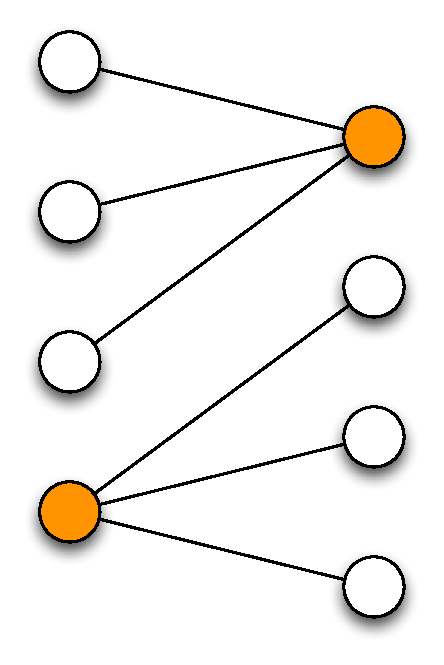
\includegraphics[width=\linewidth/3]{images/connection_graph.eps} \caption{Example of a bipartite connection graph with two concentrators of degree 3 marked as orange}
	\label{fig:bipartite_graph}
\end{figure}

In consequence of the fact that \glspl{server socket} provide a network application or service, they are likely to be contacted by several clients depending on their popularity. To this end, a socket which is contacted by a certain amount of client sockets and thus have a high degree in the connection graph is defined to be a concentrator. These concentrators are likely to offer network services and are thus \glspl{server socket}. This approach is able to detect \glspl{server socket} which are offering not only classical client-server services running on well known ports, such as web, \gls{FTP}, or \gls{SSH}, but also \gls{p2p} applications such as for example Skype and Bit-torrent super-nodes.

Extracting the concentrators form the bipartite connection graph is basically a minimum vertex cover problem which can be solved by the greedy algorithm outlined in algorithm \ref{alg:service_tracing_ss-detection}. Generally, this algorithm creates two lists for each side of the graph, one list for the internal sockets and the other for the external list. Both lists are sorted by the connection degree of the sockets. Then, the list higher degree is selected and the highest degree sockets are iteratively declared as concentrators and removed so that also all edges to other sockets are removed. Then, the lists are accordingly updated. This is done as long as there are sockets with higher degrees than $deg_{lim}$. 

% introduce minimal vertex cover problem
% greedy algorithm to solve mvcp
% recalling sockets for optimization
\begin{algorithm}[t!]
\caption{Detection of server sockets by \citet{Schatzmann:Mining,Schatzmann:Dissection, Schatzmann:Tracing}}
\label{alg:service_tracing_ss-detection}
\begin{algorithmic}
\STATE
\STATE compute list $SS_{in}$ \COMMENT{int. sockets sorted by \# ext. clients}
\STATE compute list $SS_{out}$ \COMMENT{ext. sockets sorted by \# int. clients}
\STATE
\WHILE{(deg($SS_{out}[0]$) $ > deg_{lim} $ \OR deg($SS_{in}[0]$)$ > deg_{lim}$)}
    \WHILE {(deg($SS_{in}[0]$) $ > $ deg($SS_{out}[0]$))}
        \STATE $ss$ = $SS_{in}[0]$ \COMMENT{classify $ss$ as internal server socket}
        \STATE remove $ss$ from $SS_{in}$
        \STATE update deg() for all entries of $SS_{in}$
    \ENDWHILE
    \WHILE{(deg($SS_{out}[0]$) $ \geq $ deg($SS_{in}[0]$))}
        \STATE $ss$ = $SS_{out}[0]$ \COMMENT{classify $ss$ as external server socket}
        \STATE remove $ss$ from $SS_{out}$
        \STATE update deg() for all entries of $SS_{out}$
    \ENDWHILE
\ENDWHILE
\end{algorithmic}
\end{algorithm}

\begin{figure}
	[ht] \centering
	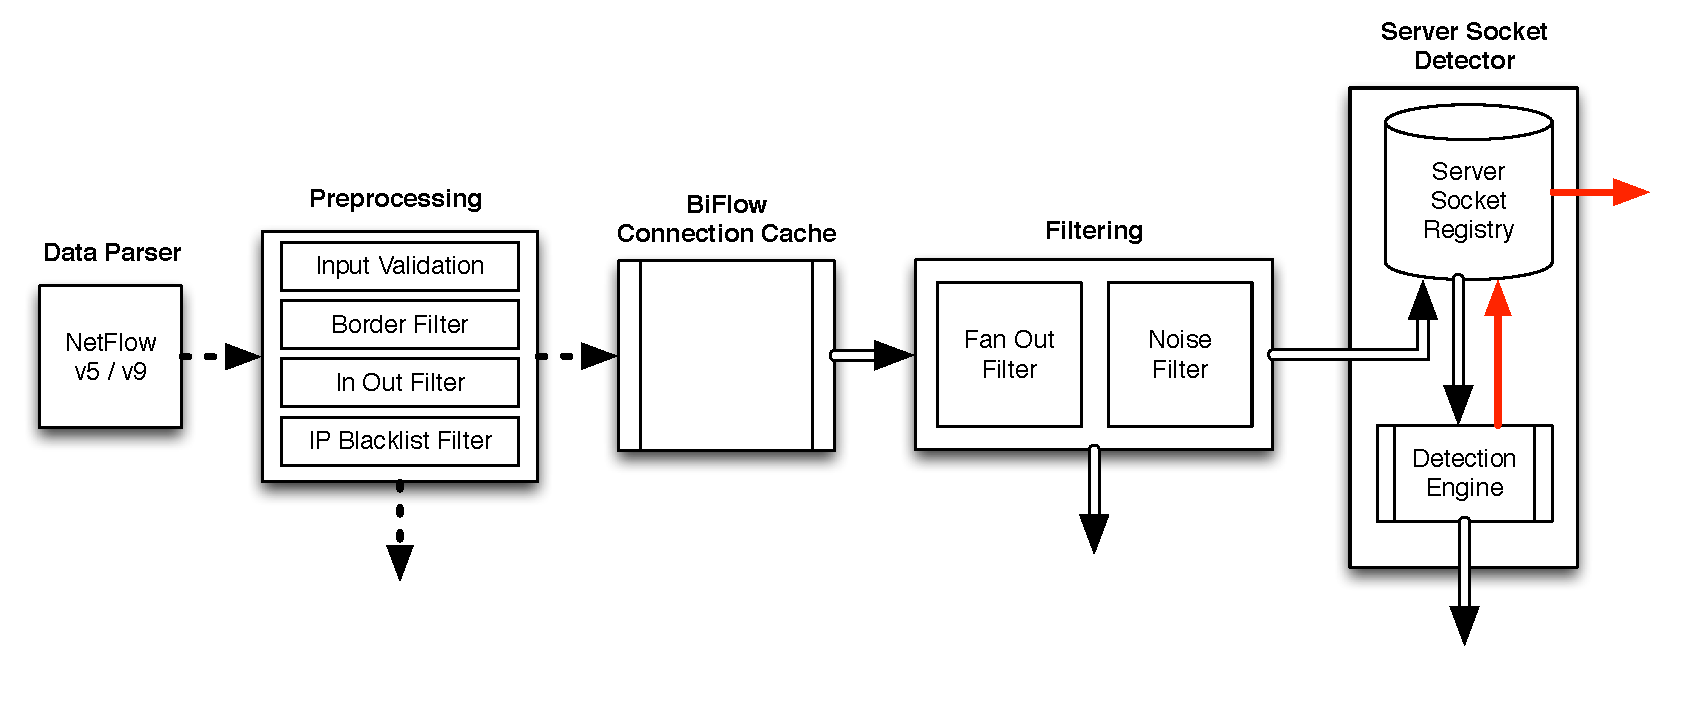
\includegraphics[width=\linewidth]{images/Detection_chain.eps}
	\caption{Processing chain for server socket detection}
	\label{fig:detection_chain}
\end{figure}

\subsection{Implementation}
Figure \ref{fig:detection_chain} illustrates the processing steps of the overall detection chain. The data parser is responsible to read the netflow data either in NetFlow v5 or NetFlow v9 format. These unidirectional flow records are then preprocessed by different blocks. While the input validator is performing some basic sanity checks of the flow data, the preprocessing filters are limiting the number of flows to the required kind of flow data. On the one hand, the border filter is removing all flow records not generated by a border router interface to efficiently prevent duplicate flow records. On the other hand, the In-Out filter is removing all non cross-border traffic, i.e., transit traffic (external to external) or entirely internal traffic (internal to internal). Furthermore, the IP blacklist filter is removing traffic towards blacklisted IP addresses or networks.

After the preprocessing, the unidirectional flows are handed to the connection cache. This connection cache is responsible for merging all related unidirectional flow record into a single bidirectional flow record during a certain caching interval. 
Two unidirectional flows are related if the source socket of one flow record match the destination socket of another flow record and vice-versa\citep{Schatzmann:Tracing}. If there is for an unidirectional flow record no other related unidirectional flow, the flow is also transformed into a bidirectional flow. Although, this bidirectional flow consists only of a single direction. All the subsequent processing is operating with these bidirectional flow records which may be of unidirectional nature. 
Furthermore, since the subsequent data processing is clock-based, a caching period $T_{cache}$ and a export period $T_{exp}$ is defined such that every $T_{exp}$ seconds all bidirectional flows records active during the last $T_{cache}$ seconds are exported and deleted from the connection cache.

After this caching step, these bidirectional flows are filtered by a fan-out filter implementing the idea of \citet{Allman:2007} to mitigate the effects of scanning and \gls{p2p} churn. This scanning filter is discussed in more detail by \citet{Schatzmann:Mining,Schatzmann:Dissection,Schatzmann:Tracing}.

Afterwards, the remaining bidirectional flow records are again reduced by the noise filter. This last filtering module is responsible to filter bidirectional flow records which does not represent a correct bidirectional connection. A correct bidirectional connection is simply defined as either a correct \gls{TCP} handshake or a reply flow as in case of \gls{UDP}. Hence, the approach of deducing correct connections is to investigate the number of packets for each direction of the bidirectional flow record, i.e., the outgoing and the incoming flow record, since there are only cross-border flows remaining due to the In-Out filter. 
If a bidirectional \gls{TCP} flow has in a single direction less than 3 packets, the filter assumes that this flow does not represent a correct connection and is removing this record. Accordingly, a bidirectional \gls{UDP} flow is required to consist of at least 1 packet for each direction. 

After these filtering steps, the remaining bidirectional flows are passed to the \emph{server socket detector} which is finally performing the \gls{server socket} detection approach previously discussed. 
Generally, the \emph{server socket detector} is build from two main parts. On the one side, there is the \emph{server socket registry} which is containing all already known \glspl{server socket}. 
On the other side, the detection engine implements the \gls{server socket} detection algorithm.

At first, the sockets of all bidirectional flows are queried against the current \emph{server socket registry} for checking if they are already known. 
If this is the case, the corresponding bidirectional flow records are removed and only the remaining flow records are passed to the detection engine to increase the efficiency of the detection algorithm. 
The detection engine builds the bipartite connection graph and is detecting the concentrators of it.
These detected \glspl{server socket} are then passed to the \emph{server socket registry} so that these sockets may be recalled afterwards.

Finally, the \emph{server socket registry} is able to output all detected \glspl{server socket} of the observation period.

%%%%%%%%%%%%%%%%%%%%%%%%%%%%%%%%%%%%%%%%%%%%%%%%%%%%%%%%%%%%%%%%%%%%%%%%%%%%%%%%
% MONITORING OF SERVER SOCKETS
%%%%%%%%%%%%%%%%%%%%%%%%%%%%%%%%%%%%%%%%%%%%%%%%%%%%%%%%%%%%%%%%%%%%%%%%%%%%%%%%
\newpage
\section{Monitoring of Server Sockets
\label{section:socket_tracking}}

The previous section outlined the approach of detecting \glspl{server socket}. This section covers the approach of monitoring flow data and generating statistical information such that some characteristics and properties of the detected \glspl{server socket} can be assessed as further outlined in section \ref{section:characterization}.

\subsection{Server Socket Statistics}

Generally, during the monitoring steps all information required to characterize the stability, visibility and popularity have to be captured. This kind of information is denoted as \gls{server socket} statistics.

To this end, all flows originated from a \gls{server socket} or flows which are destined to \glspl{server socket} are monitored for compiling these \gls{server socket} statistics. In contrast to the detection approach, all flows towards a known \gls{server socket} have to be considered, since they have to be accounted to the statistics.

Since the flow-level data is usually discretely slotted by chunks of size of the export period $T_{exp}$, \gls{server socket} statistics records can be accounted on a time slot basis as well. A \gls{server socket} statistics record contains the following information per time slot:
\vbox{
\begin{itemize}
	\item number of bidirectional connections
	\item number of outgoing unidirectional connections
	\item number of incoming unidirectional connections
\end{itemize}
}

In a second step, the statistics records of each discrete time slot can be aggregated in such a way that the information of the activity within a certain time slot is kept. Thus, the overall \gls{server socket} statistics record contains the following entries:

\vbox{
\begin{itemize}
	\item sum of bidirectional connections of each time slot
	\item sum of outgoing unidirectional connections of each time slot
	\item sum of incoming unidirectional connections of each time slot
	\item number of days with connections
	\item number of discrete time slots with connections
	\item timestamps of discrete time slots with connections
\end{itemize}
}

\subsection{Traffic Statistics}

Besides the individual \gls{server socket} statistics report, overall traffic statistics are accounted, mainly for deducing knowledge of how good the monitoring capability of the \glspl{server socket} in the \emph{server socket registry} is. For this reason, each flow which belongs to a \gls{server socket} and is present in the \emph{server socket registry} is denoted as monitored. Hence, flows which do not belong to a \gls{server socket} are accounted as not monitored.

Moreover, all unmonitored flows can be further investigated for a better understanding of the type of this unmonitored traffic. This can be done on the following three scopes:
\begin{itemize}
	\item protocol level
	\item port level for \gls{UDP} and \gls{TCP} flows
	\item location of the connection end-points
\end{itemize}

The first scope captures statistical information of the problem that \glspl{server socket} are only defined for protocol \gls{TCP} and \gls{UDP}, hence all flows with another protocol are per definition unmonitored.

In a second step, there are statistics generated for all unmonitored \gls{TCP} or \gls{UDP} flows. There are various reasons for unmonitored flows, mainly related to the detection approach outlined in section \ref{section:socket_detection}. 
In most of the cases, the sockets are not contacted by enough clients, therefore, they are not detected as concentrators and in consequence of that not recognized as \glspl{server socket}. 
Furthermore, scanning activity is also a major contributor to those unmonitored flows, since scanning traffic and other non-legitimate traffic is removed before the \gls{server socket} detection is performed. Consequently, these scanned sockets are not detected as \glspl{server socket}, in case there is no legitimate traffic towards these sockets. Nevertheless, this scanning traffic is considered in this monitoring phase as well.

On the one hand, there is the possibility to account for each port of the unmonitored flows which will lead to very detailed statistical information about missed sockets. However, this comes at the price of an inefficient processing and higher memory usage.

On the other hand, the flows can be categorized by port ranges. In the thesis at hand, there are just two ranges defined for this categorization:

\begin{itemize}
	\item low port: 0-1023
	\item high port: 1024-65365
\end{itemize}

These categories are further divided by the location of the socket either internal or external and thus involving the third scope. Hence, the unmonitored \gls{TCP} and \gls{UDP} flows by the following four categories:

\vbox{
\begin{itemize}
	\item external port high, internal port high
	\item external port high, internal port low
	\item external port low, internal port high
	\item external port low, internal port low
\end{itemize}
}

All these general traffic statistics allow to deduce insights about the properties of the detection process by learning what is missed. Moreover, these general traffic statistics are revealing information about the properties of the current \gls{server socket} set with respect to traffic representation and thus about some properties of this set.

\subsection{Implementation}

Figure \ref{fig:monitoring_chain} shows the modular implementation of the \gls{server socket} monitoring chain. Comparing the monitoring chain to the detection chain from figure \ref{fig:detection_chain} it is clearly visible that the modules up to the bidirectional connection cache are shared. 
However, in the monitoring chain there are no fan-out filter and noise filter applied. T
his is because every traffic destined to a \gls{server socket} should be considered, therefore, no bidirectional flow records are filtered before accounting them. 
The \emph{server socket monitor} is accounting the general traffic statistics as well as the individual \gls{server socket} statistics.

First of all, the bidirectional flow records are separated into those belonging to a known \gls{server socket}, denoted as monitored traffic, and those not belonging to known \gls{server socket}, denoted as unmonitored traffic. To be more precisely, this is done by querying the \emph{server socket registry} which is loaded with previously detected \glspl{server socket}. Then, the traffic monitor investigates the monitored and unmonitored traffic for generating the overall traffic statistics.
Furthermore, it examines the unmonitored traffic even more closely for deducing knowledge about the other traffic statistic scopes as protocol, ports and location.

\begin{figure}[hb]
	\centering
	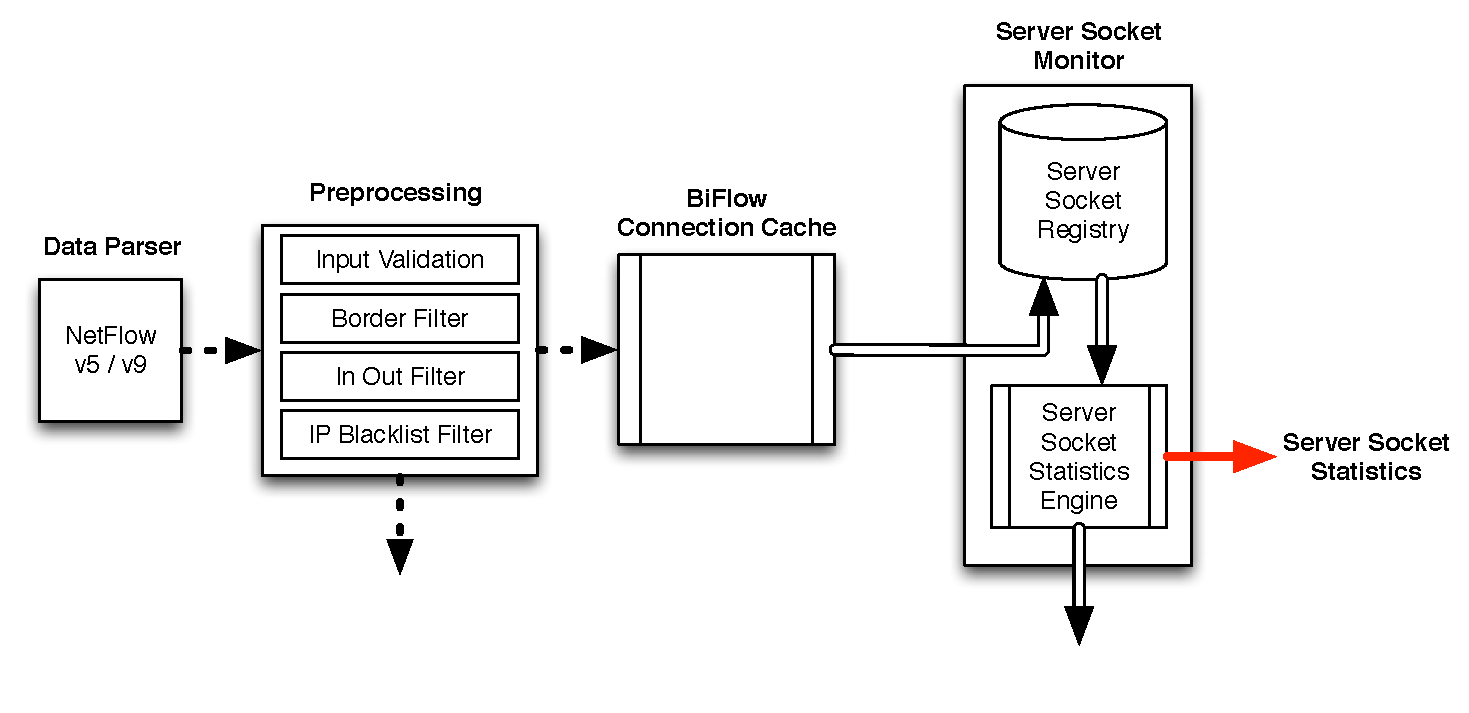
\includegraphics[width=\linewidth]{images/TrackingChain.eps}
	\caption{Processing chain for the server socket monitoring}
	\label{fig:monitoring_chain}
\end{figure}

%%%%%%%%%%%%%%%%%%%%%%%%%%%%%%%%%%%%%%%%%%%%%%%%%%%%%%%%%%%%%%%%%%%%%%%%%%%%%%%%
% CHARACTERIZATION SERVERSOCKETS
%%%%%%%%%%%%%%%%%%%%%%%%%%%%%%%%%%%%%%%%%%%%%%%%%%%%%%%%%%%%%%%%%%%%%%%%%%%%%%%%
\newpage
\section{Characterization of Server Sockets
\label{section:characterization}} 

The main interest of this thesis is to characterize \glspl{server socket} by their \textbf{stability}, their \textbf{visibility} and their \textbf{popularity}. These properties address the following characteristics of a \gls{server socket}:

\vbox{
\begin{itemize}
	\item \textbf{Stability:} How stable is the \gls{server socket} regarding its responsiveness or availability?
	\item \textbf{Visibility:} How frequently is the \gls{server socket} contacted?
	\item \textbf{Popularity:} How many distinct clients or sockets are contacting the \gls{server socket}?
\end{itemize}
}

These three characteristics are directly deducible from the statistics observed by the passive monitoring technique outlined in \ref{section:socket_tracking}. In the following, the three characteristics are briefly discussed.

\subsection{Stability of a Server Socket}
Because of the definition and its detection approach a \gls{server socket} is offering a bidirectional service which means that the client and the \gls{server socket} are both sending packets. 
Usually, a client socket is opening the connection to a \gls{server socket} which will reply in return to this request. 
Generally, this also holds for \gls{p2p} applications as for example bit torrent. Therefore, a \gls{server socket} -- or the communication of it -- can be characterized as stable if it responds to all connection attempts. 
If a connection attempt to a \gls{server socket} is answered by the \gls{server socket}, the connection is bidirectional, otherwise it is an unidirectional flow destined towards the \gls{server socket}.

Thus, the overall stability \gls{server socket} or availability of its service can be approximated by the ratio of the bidirectional flows to all flows destined to this \gls{server socket}, i.e., the bidirectional and the unidirectional incoming. 
This ratio is referred as a \gls{server socket} \textbf{stability} and is mathematically defined by equation \ref{eq:ratio}.
\begin{equation}
	\text{Stability}(\text{Socket}_i) = \frac{\text{bidirectional flows}(\text{Socket}_i)}{\text{bidirectional flows}(\text{Socket}_i) + \text{unidirectional flows}_{in}(\text{Socket}_i)}
	\label{eq:ratio}
\end{equation}

Hence, a \gls{server socket} with a stability of 1 does only have bidirectional connections and thus, replies to all connection attempts. 
On the other side, a stability of 0 indicates that there are only connections attempts by client sockets, but the \gls{server socket} has never replied upon these requests. 
Unbalanced outgoing connections from the \glspl{server socket} are indicating a client error or scanning activities of clients with spoofed (internal) source address which are not observed by the monitoring system. 
Therefore, these unbalanced outgoing connections are not considered for determining the stability ratio at all.

\subsection{Visibility of a Server Socket\label{subsection:visibility}}

% discrete time slots activities of a socket, per day, per 5min slot?
% distribution is heavy-tailed, alot of sockets only rarely connected => due to scanning? due to malware?
The monitoring process of the \glspl{server socket} is done passively, thus if a \gls{server socket} is visible in the flow-level data of a certain time period, the \gls{server socket} is active during that time. Hence, the visibility of a \gls{server socket} during a certain time interval $[t,t+\Delta{t}]$ is a binary measure, either inactive in case it is not visible or active in case it is visible in the data set. Equation \ref{eq:visibility} defines the visibility of a socket during the time interval $[t,t+\Delta{t}]$:
\begin{equation}
	\text{Visibility}_t(\text{Socket}_i,t+\Delta{t}) = \left\{
	\begin{array}{l l}
		1 & \quad \text{if $\text{Socket}_i$ is active during $t+\Delta{t}$}\\
		0 & \quad \text{if $\text{Socket}_i$ is not active during $t+\Delta{t}$}\\
	\end{array}
	\right.
	\label{eq:visibility}
\end{equation}

In consequence, there are different granularities $\Delta{t}$ to define the visibility of a \gls{server socket}. On the one hand, the most fine-grained resolution is just the flow-level data cache export period $T_{exp}$. In most of the cases, this flow-level data cache export period $T_{exp}$ is set to 300 seconds. This most fine-grained resolution is referred to as the \emph{time slot} resolution, since the entire processing is based on such discrete data chunks, containing all flows active during this time period. 
On the other hand, there are several more coarse-grained resolutions of the visibility possible. An obvious is resolution of a day, i.e., $\Delta{t} = 86400$s.

Furthermore, the visibility of a \gls{server socket} can be extended from a single time period to the overall observation time, i.e., a week long trace, by summing up the individual visibilities of each time slot as shown in equation \ref{eq:visibility_sum}.

\begin{equation}
	\text{Visibility}(\text{Socket}_i) = \sum_{t} \text{Visibility}_t(\text{Socket}_i,t+\Delta{t})
	\label{eq:visibility_sum}
\end{equation}

However, this summing approach exacerbate the comparison between different observations since it represents the visibility in absolute terms. 
Therefore, an even better metric for the visibility of a \gls{server socket} is to average the individual $\text{Visibility}_t(\text{Socket}_i,t+\Delta{t})$ as outlined by equation \ref{eq:visibility_avg}.
This normalizes the visibility to a value in the range between 0 and 1, representing the ratio of its visibility to the maximum visibility possible. 
Thus, a value of 1 means that the socket is visible in every single time slot and a value of 0 that the socket was never active.

\begin{equation}
	\overline{\text{Visibility}}(\text{Socket}_i) = \frac{\sum_{t} \text{Visibility}_t(\text{Socket}_i,t+\Delta{t})}{\sum_{t}1}
	\label{eq:visibility_avg}
\end{equation}

\subsection{Popularity of a Server Socket}

% number of flows / clients?.. degree of Server Socket
Besides the visibility of a \gls{server socket}, its popularity is another major key characteristics. 
Whereas the visibility of a \gls{server socket} defines how frequent a socket is contacted by at least one connection endpoint, the popularity of a \gls{server socket} is defined by the number of connection attempts of client sockets during a certain period of time. 
The popularity of \gls{server socket} can be deduced by various metrics such as the number of flows, bytes, or clients.

%%%%%%%%%%%%%%%%%%%%%%%%%%%%%%%%%%%%%%%%%%%%%%%%%%%%%%%%%%%%%%%%%%%%%%%%%%%%%%%%
% Smart Traffic Selection using Server Sockets Sets
%%%%%%%%%%%%%%%%%%%%%%%%%%%%%%%%%%%%%%%%%%%%%%%%%%%%%%%%%%%%%%%%%%%%%%%%%%%%%%%%
\newpage
\section{Smarter Traffic Selection using Server Sockets Sets 
\label{section:ses_traffic_selection}}

% explain briefly the approach / adjustments to FACT
Originally, \gls{FACT} applies a port-based heuristic for selecting the  examination traffic.  
In detail, \gls{FACT} selects in a first step all traffic towards an external  \gls{TCP} port 80 originated from an internal client high port. 
Generally, this kind of traffic is denoted as the reflector traffic. 
Then, \gls{FACT} examines each connection from the reflector traffic if it is  balanced or unbalanced, thus creating an initial set of potential events. 

\begin{figure}
	[!b] \centering
	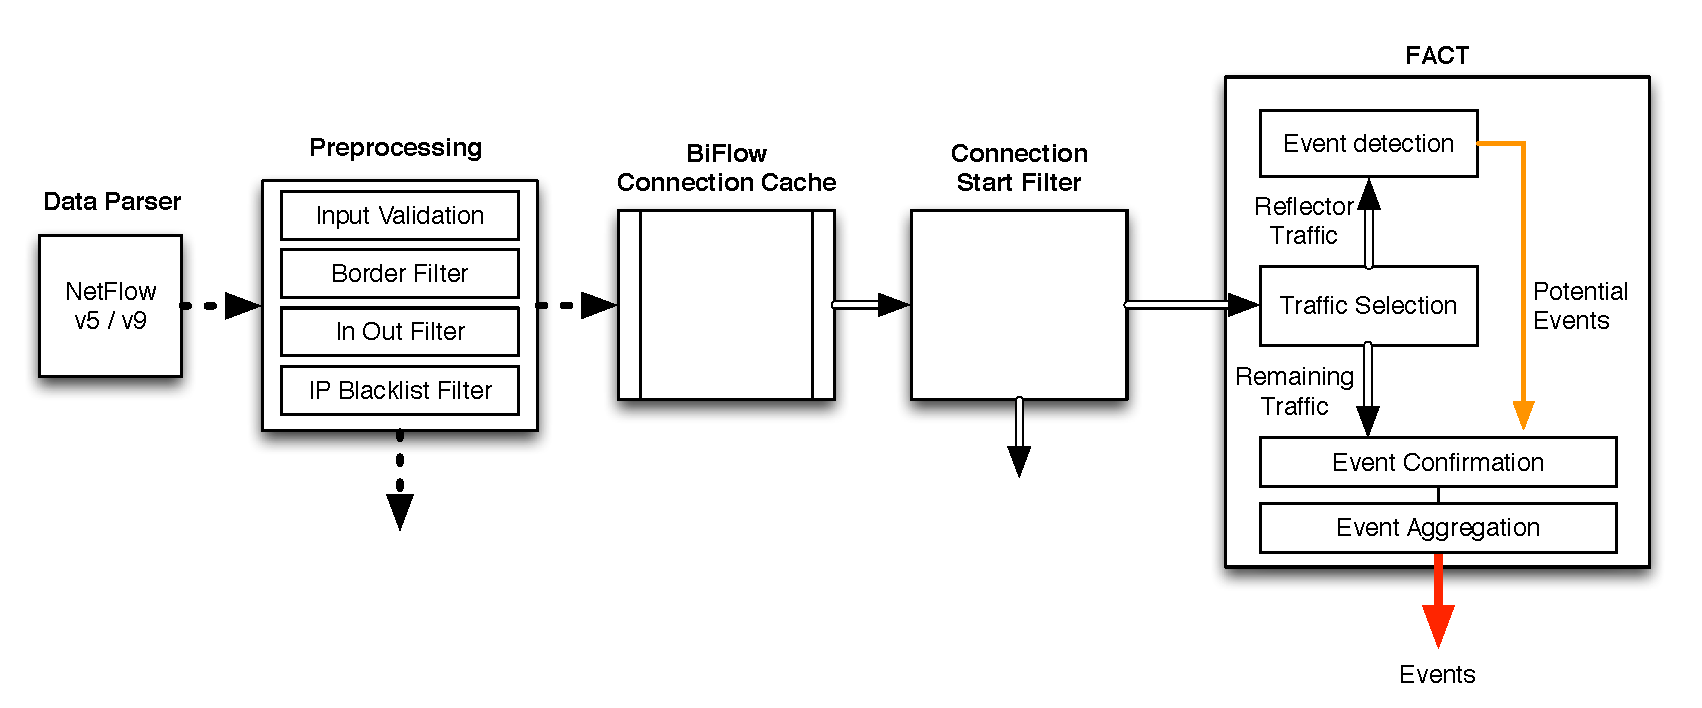
\includegraphics[width=\linewidth]{images/FACT.eps}
	\caption{Processing chain for FACT} 
	\label{fig:fact_chain} 
\end{figure}

In a second step, all potential events inferred by the reflector traffic are  double-checked with the remaining traffic if a potential event is indeed a  event. 
Only if there are no successful connections at all, i.e., all connections  are unbalanced, a host, network, or prefix is declared as unreachable. 
Otherwise, if there is other traffic towards these hosts, networks, and prefixes with balanced connections, the potential event is obviously not confirmed and thus removed from the event list. 

Since the \gls{server socket} approach aims to replace the port-based heuristic,  only the generation of the reflector traffic set must be adjusted. 
The further processing steps remain exactly the same. 
Figure \ref{fig:fact_chain} illustrates the \gls{FACT} processing chain and makes clear that only the block of the traffic selection must be adjusted to examine traffic towards \glspl{server socket} as reflector traffic. 
This is achieved by loading the \gls{server socket} registry with a set of \glspl{server socket}. 
Then, the adjusted traffic selection is querying the server socket registry if the external socket is a known \gls{server socket}. 
If this is the case, the flow is added to the reflector traffic, otherwise to the remaining traffic. 

\subsection{Selecting Suitable Server Sockets Sets\label{section:ses_selection}}
% outline that this is a optimization problem which is approximated by several 
% socket sets however not guaranteed to be optimal
% coverage network space / problem space 
By adjusting the traffic selection of \gls{FACT} with \gls{server socket} sets,  some essential properties of \gls{FACT} as the observed network coverage or the event sensibility are directly dependent on properties of the chosen \gls{server socket} set. 

Because \gls{FACT} detects only network outage events which are firstly detected  with the reflector traffic and then not whitelisted by the remaining traffic, it  is able to detect only network outages of prefixes which have at least one known  server socket that is located in this prefix. This means that FACTs observation  coverage of networks is completely defined by the network/prefix coverage of the  chosen \gls{server socket} set. 

Obviously, it makes no sense to select for example the 10 most popular sockets if they are all located in the same network and prefix, because this set would just achieve a network coverage of 1 network/prefix. 
Hence, the network coverage can be optimized by selecting the best socket of these 10 and then select 9 different sockets which are all located in different networks/prefixes. 
By doing so, the network coverage can be increased. However, if a selected  \gls{server socket} is not contacted during an observation period the observation coverage of this network is lost, unless there is another contacted socket located in this network. 
This shows that the selection of \glspl{server socket} is cumbersome and directly influences the observation capabilities of FACT. It also shows the importance of the visibility and popularity characteristics of \glspl{server socket} with respect to the selection in a \gls{server socket} set. 

A popular \gls{server socket} which is always contacted by at least one client is able to cover the entire network, because even if this socket is not reachable during an observation period the network is further investigated by the remaining traffic. 
This is because the unbalanced connection of this \gls{server socket} will trigger a potential event which is then confirmed or whitelisted by the  remaining traffic towards this network. 
Otherwise, if a socket is not popular and only rarely visible, it will not generate a potential event, and hence, the event is not detected at all, even if there is a lot of unbalanced traffic towards this network contained in the remaining traffic. 

Therefore, the selection of the \glspl{server socket} is basically an optimization problem. 
The goal is to select those sockets with good stability, popularity and visibility characteristics without loosing to much network coverage. 
This problem can even be harder if the number of sockets is limited, then the socket density of each network must be considered, so that only the few best sockets located in a single network are selected.
It can even make sense to include not perfectly 
stable sockets if they increase the network coverage, especially if they have a good visibility and popularity.
